\documentclass{AlstomLibrary} 

\title{Outil de création de tableaux graphiques \TT}
\titlehead{Version du document : \version}
\author{Guillaume MANCIET}
\newcommand{\version}{0.3}
\newcommand{\progname}[1]{\textit{#1}}

%\newcommand{\modulename}[1]{\texttt{#1}}

\usepackage{xcolor}
\usepackage{rotating}
\usepackage{listings}
\lstset{ % general style for listings
   numbers=left
   , tabsize=2
   , frame=single
   , breaklines=true
   , basicstyle=\ttfamily
   , numberstyle=\tiny\ttfamily
   , framexleftmargin=13mm
   , backgroundcolor=\color{gray}
   , xleftmargin=12mm
   %, frameround={tttt}
   , captionpos=b
}
\lstdefinestyle{xslt}
{
    emph={xsl,template,variable,param,for,each,apply,templates,with,param}
    , emphstyle=\color{magenta}
    , emph={[2]match, select, name, mode}
    , emphstyle={[2]\color{cyan}}
}

\usepackage{makeidx}

\newcommand{\INTERVLEGEND}{\index{Propriétés d'intervalle!LEGEND}\texttt{LEGEND}}
\newcommand{\PROPSIZEX}{\index{Propriétés graphiques!SIZE\_X}\texttt{SIZE\_X}}
\newcommand{\PROPSIZEY}{\index{Propriétés graphiques!SIZE\_Y}\texttt{SIZE\_Y}}
\newcommand{\PROPPOSX}{\index{Propriétés graphiques!POS\_X}\texttt{POS\_X}}
\newcommand{\PROPPOSY}{\index{Propriétés graphiques!POS\_Y}\texttt{POS\_Y}}
\newcommand{\TT}{{\progname{TrainTracer}} }

\makeindex

\begin{document}

\maketitle

\addcontentsline{toc}{part}{Table des matières}
\tableofcontents
\setcounter{tocdepth}{2}
\listoftables
\listoffigures

%\tableofcontents

%\listoffigures 	% to produce list of figures
%\listoftables 	% to produce list of tables

\chapter{Introduction}

Cet outil vise à améliorer la conception des tableaux de bord graphiques utilisés par \TT, en permettant des actions non proposées, comme par exemple le placement par coordonnées, la rotation, la mise à l'échelle. Il est particulièrement recommandé pour créer des tableaux de bords comportant beaucoup d'éléments identiques, en terme de visualisation.

L'outil nécessite un temps de préparation important lié aux informations requises par le fichier CSV, particulièrement:
\begin{itemize}
\item chemin et nom des variables;
\item nom des images a placer;
\item coordonnées exactes de images à placer.
\end{itemize}

Cependant, la maîtrise du fichier CSV via \textsl{ un éditeur adapté} rend les opérations beaucoup plus rapides. Les exemples réalisés en annexe sont ainsi réalisés en une demi-journée, dont près de la moitié du temps consacré est lié à la création des images.

\chapter{Prérequis}

\section{Outils nécessaires et recommandés}

\subsection*{Requis: \progname{Perl}}

Pour pouvoir être exécute, le script a besoin de \progname{Perl}. Ceci est fourni en standard si vous avez le client de \progname{Clearcase} d'installé. Ceci peut également être fourni par le client lourd de \progname{ClearQuest}.

\subsection*{Recommandé: Éditeur de fichier CSV}

Les fichiers CSV utilisés comme données sources peuvent être édités simplement avec des outils comme \progname{Excel}.

\subsection*{Recommandé: Éditeur d'images}

Les images utilisées comme fond peuvent être édités assez simplement en utilisant un éditeur d'images adapté, ayant à minima les fonctionnalités d'affichage des coordonnées, qui vous seront utiles pour compléter le fichier CSV. L'outil utilisé sera ici \progname{Paint.NET}. 

\subsection*{Recommandé: \TT}

L'éditeur originel des tableaux de bord graphique reste requis pour valider les tableaux de bords graphiques en condition réelles. Les anomalies liées à \TT doivent être prises en compte lors de la conception.

\section{Connaissances requises}

\textbf{Pour la suite du document, on considérera comme acquise la création manuelle de tableaux de bords graphiques via \TT}.

\chapter{Utilisation}

\section{Configuration du programme}

La configuration est un point important mais rapide. Celui-ci permet d'indiquer au programme les chemins par défaut des variables, les fichiers à utiliser, le nom des tableaux de bords, et d'autres points. La configuration est effectuée via le fichier \texttt{config.xml} du répertoire \texttt{config}, où sont décrites toutes les options nécessaires (fichier commenté).

\section{Éléments graphiques}

\subsection{Éléments statiques}

\subsubsection{Images statiques}

Les images statiques permettent de présenter des informations à l'utilisateur, au travers d'une image. Elles n'évoluent pas au fil du temps et leur couleur n'est pas configurable.

La représentation sous \TT est définie à la figure~\vref{TT_ImageControl}.

\begin{figure}\centering

\includegraphics[scale=1]{TT_ImageControl.png}
\caption{Représentation de l'image dynamique sous \TT}\label{TT_ImageControl}
\end{figure}

\subsubsection{Textes statiques}

Les images statiques permettent de présenter des informations textuelles simples à l'utilisateur. Elles n'évoluent pas au fil du temps et leur couleur n'est pas configurable.

La représentation sous \TT est définie à la figure~\vref{TT_Label}.

\begin{figure}\centering
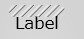
\includegraphics[scale=1]{TT_Label.png}
\caption{Représentation du texte dynamique sous \TT}\label{TT_Label}
\end{figure}

\subsection{Éléments dynamique}

\subsubsection{Images dynamiques}

Les images dynamiques permettent d'associer une ou plusieurs images à la valeur d'une variable. Les images représentant les états doivent être définis conformément à la section~\vref{SECT_DYN_INTERVAL}.

La représentation sous \TT est définie à la figure~\vref{TT_ImageViewVariable}.

\begin{figure}\centering
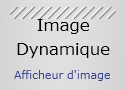
\includegraphics[scale=1]{TT_ImageViewVariable.png}
\caption{Représentation de l'image dynamique sous \TT}\label{TT_ImageViewVariable}
\end{figure}

\subsubsection{Textes dynamiques}

Les textes dynamiques permettent d'afficher la valeur d'une variable. Celui-ci a la faculté de changer de couleur en fonction des intervalles que vous aurez définis. Les couleurs représentant les états doivent être définis conformément à la section~\vref{SECT_DYN_INTERVAL}.

La représentation sous \TT est définie à la figure~\vref{TT_SimpleView}.

\begin{figure}\centering
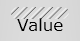
\includegraphics[scale=1]{TT_SimpleView.png}
\caption{Représentation du texte dynamique sous \TT}\label{TT_SimpleView}
\end{figure}

\subsection{Propriétés des éléments graphiques}

Les champs à renseigner pour les éléments utilisables sont décrits dans le tableau~\vref{TAB_PROPS_ELEMENT}.

\begin{table}\centering
\begin{tabular}{@{}lp{7cm}cccc}  \toprule%{@{}llll@{}}
Texte & Description & \begin{sideways}Image statique\end{sideways} & \begin{sideways}Texte statique\end{sideways} & \begin{sideways}Image dynamique\end{sideways} & \begin{sideways}Texte dynamique\end{sideways} \\
\midrule
\texttt{ELEMENT\_TYPE} & Nom de l'élément à créer. Si ce champs est vide, les autres champs ne sont pas lus. & O & O & O & O \\
\PROPPOSX  & Position absolue de l'élément selon l'axe des X. & O & O & O & O \\
\PROPPOSY  & Position absolue de l'élément selon l'axe des Y. & O & O & O & O \\
\PROPSIZEX  & Dimensions en X de l'élément. & O & F & O & F \\
\PROPSIZEY  & Dimensions en Y de l'élément. & O & F & O & F \\
\texttt{LOCKED} & Verrouillage de l'objet, rendant son déplacement accidentel impossible. & F & F & F & F \\
\texttt{SCALE} &  Rapport d'échelle. Ce rapport est calculé après appliquer les dimensions en X et Y. & F & F & F & F \\
\texttt{ANGLE} &  Angle de rotation appliqué à l'élément en degré. & F & F & F & F \\
\texttt{TEXT} &  Texte de l'élément. &  & O &  &  \\
\texttt{IMAGE\_PATH} &  Chemin vers l'image à utiliser. &  &  & O &  \\
\texttt{PATH} &  Chemin vers la variable à utiliser. &  & O &  & O \\
\texttt{RNGE[...]} & Utilisation des intervalles dynamiques. & & O & & F \\
\bottomrule
\end{tabular}
\caption{Tableau des propriétés des éléments.}\label{TAB_PROPS_ELEMENT}
\end{table}

\section{Définition des intervalles dynamiques} \label{SECT_DYN_INTERVAL}

\subsection{Système d'intervalles sous \TT}

Les effets dynamiques (de texte, d'image, de cellules) sur \TT reposent intégralement sur un  système d'intervalle, présenté à la figure~\vref{TT_CUSTOM_DISPLAY}. C'est le tableau qui apparaît lorsque l'on clique sur l'affichage personnalisé, dans la fenêtre d'édition des variables. Ainsi, dans la figure~\vref{TT_CUSTOM_DISPLAY}, trois intervalles sont définis : $[0-0]$, $[10-12]$ et $[13-255]$, chaque intervalle ayant des propriétés potentiellement différentes.

\begin{figure}\centering
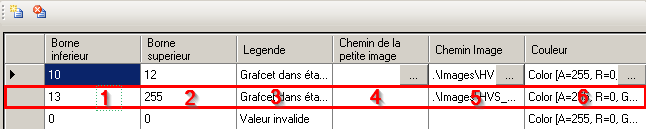
\includegraphics[scale=0.5]{TT_Custom_display.png}
\caption{Système d'intervalles de \TT}\label{TT_CUSTOM_DISPLAY}
\end{figure}

\subsection{Transcription de ce système dans l'outil}

Les colonnes du fichier CSV doivent respecter un canevas particulier, afin d'être reconnu par l'outil. Chaque colonne d'un intervalle est caractérisée par l'emploi du mot clé \lstinline{RNGE[<valeur_min>-<valeur_max>]_<mot_cle>}, suivi par l'un des mots clés présentés au tableau~\vref{TAB_PROPS_INTERVAL}. Il n'est pas nécessaire de définir tous les éléments.

\begin{table}\centering
\begin{tabular}{@{}llp{7cm}cc}  \toprule%{@{}llll@{}}
Champ & Texte & Description & G\footnote{Propriété apparaissant dans la visualisation graphique des tableaux de bord} & T\footnote{Propriété apparaissant dans la visualisation tabulaire des tableaux de bord} \\
\midrule
\#1 & \texttt{valeur\_min}  & Intervalle inférieur. Si c'est un booléen, utiliser 0 et 1. & & \\
\#2 & \texttt{valeur\_max}  & Intervalle supérieur. Peut être égal à l'intervalle inférieur. & & \\
\#3 & \INTERVLEGEND  & légende visible en pointant l'élément graphique. & X & \\
\#4 & \texttt{SMALL\_IMAGE}  & Représentation dans le tableau de bord tabulaire. & & X \\
\#5 & \texttt{IMAGE} &  Représentation dans le tableau de bord graphique. & X & \\
\#6 & \texttt{COLOR} &  Couleur utilisée dans le tableau de bord graphique pour colorer le texte en fonction des valeurs. & X & X \\
\bottomrule
\end{tabular}
\caption{Tableau des propriétés liées aux intervalles.}\label{TAB_PROPS_INTERVAL}
\end{table}

\chapter{Exemples}

Les différentes situations décrites dans le fichier \texttt{Exemples.xlsx} présent dans le répertoire d'exemple. Des commentaires sont éventuellement placés aux endroits importants. Les différentes situations sont présentées au tableau~\vref{TAB_EXAMPLES}.

\begin{table}[htbp]\centering
\begin{tabular}{@{}lp{4.5cm}p{7cm}}  \toprule%{@{}llll@{}}
Onglet & Description courte & Description  \\
\midrule
\textbf{Img Dyn} & Image dynamique sur un booléen  & Présentation d'une images dynamique simple basée sur un booléen (deux états). \\
\textbf{Img Dyn mul} & Image dynamiques identiques multiples & Présentation de plusieurs images dynamiques simples ET identiques basée sur une même variable.  \\
\textbf{Img Dyn Rep mul} & Variable unique avec plusieurs représentations  & Astuce pour avoir plusieurs représentations d'une même variable.  \\
\textbf{Img Dyn entier} & Image dynamique sur un entier  & Présentation d'une images dynamique simple basée sur un entier (plusieurs états).  \\
\textbf{Var sans rep} &Variable sans représentation graphique &  Présentation d'une variable apparaissant dans le tableau de bord tabulaire uniquement. \\
\bottomrule
\end{tabular}
\caption{Tableau des exemples}\label{TAB_EXAMPLES}
\end{table}

\chapter{Foire aux questions}

\section*{Je n'arrive pas a superposer mes images avec le fond}

\TT déforme légèrement les images (quelques pixels). Par conséquent, il peut être nécessaire de procéder à un ajustement manuel des coordonnées (\PROPPOSX, \PROPPOSY) et/ou de l'échelle (\texttt{SCALE}).

\end{document}

